\documentclass{article}

\usepackage{amsmath}
\usepackage{amssymb}
\usepackage{graphicx}
\usepackage{authblk}
\usepackage{float}
\usepackage{graphicx}
\usepackage[colorinlistoftodos,prependcaption,textsize=tiny]{todonotes}
%\graphicspath{ {c:/Users/mjutras/TeXworks/images/} }
\graphicspath{ {images/} }



\author[1]{Deon Burchett, PhD}
\author[2]{Brady Collea}
\author[3]{Melanie Jutras}
\author[4]{Les Servi, PhD}
\author[5]{Randy Paffenroth, PhD}

\affil[1,2,3,4]{The MITRE Corporation}
\affil[5]{Worcester Polytechnic Institute}

\title{Minimizing the Burden of Measuring Healthcare Data with Robust Sparse PCA}
\date{}

\begin{document}



\maketitle

\section{Introduction}
\todo[inline]{I pulled some content from previous Academy Health abstract with the exception of findings. Check to see if I missed anything from that abstract that we ought to include}
\subsection{Background}
Requiring metrics for the evaluation of healthcare systems and initiatives is necessary in order to improve healthcare safety, quality and value. However, collecting and managing healthcare quality measures is expensive and time consuming. Additionally,  proposed sets of health metrics are often larger than necessary. Proposed metrics often do not account for redundancy of information between metrics, cost of gathering metrics, or reliability of various metrics. [Ref AcademyHealthAbstract]  Our research was performed initially with synthetic data where ground truth is known and error can be precisely calculated. These methods were then applied to health metrics obtained from public use files containing actual health metrics collected over a period of one year.The methods proposed herein can be used to solve this government problem by reducing burden and improving quality.
\subsection{Summary of Methods}
\todo[inline]{2-3 paragraph summary of methods}
\subsubsection{Traditional PCA}
\todo[inline]{a. No anomaly handling: Matt's exhaustive search of greedy algorithm}
Traditional Principal Components Analysis (PCA) works well for dimensionality reduction, however, it is often seen as difficult to interpret.  The reason for this is that PCA produces a set of results which are linear combination of features.  This is useful for understanding the rank or underlying dimension, but does not help to select specific measures from a set of attributes. Additionally, and an important note for this research, is that PCA is extremely sensitive to ouliers.  One outlier in the data can completely change the results.
\subsubsection{Robust PCA Convex Optimization Approach}
The Convex Optimization approach is based on Robust Principal Component Analysis (RPCA).  The RPCA approach will both remove anomalies and provide a low rank approximation of the original data. This is accomplished with a combination of a nuclear norm and a one norm whcih is regularized by a tuning parameter, $\lambda$ to induce sparsity. The Robust PCA formulation is as follows.

\begin{equation}
\min_{L,S} ||L||_* + \lambda ||S||_1    s.t. L + S = M
\label{RPCA}
\end{equation}

Approximation methods are used as implemented in the dimredu python package and available as open source here.
\todo[inline]{I don't know how a python package is usually referenced}
 
\subsubsection{Robust PCA Combinatorial Approach}
\todo[color=blue,inline]{Ok, this is important.  We are not actually doing any Sparse PCA!?   This indicates we are just doing Robust PCA.   That does agree with my memory, now that I think about it.  This makes things easier, but I am not sure what the combinatorial approach is anymore.}
\todo[inline]{Insert Deon's Problem Formulation here}

\subsection{Contribution}
The main contribution of this research toward the problem at hand is to provide various methods which will both remove anomalies and provide a low rank approximation of the original data.  This results in significant reduction of mean squared errors (MSE) as will be shown in the results section.The impact of this research is the potential to minimize costly burden of obtaining healthcare quality data. This is especially beneficial when there is minimal information gained by the collection of the excess data. We have enhanced existing work to create fast algorithms for solving this government problem. Complete technical details of our research can be found in reference [newPaper]
\section{Analysis}

Data analysis was performed on both synthetic and real world data sets which will be described in the sections below. Analysis of synthetic data is particularly useful as we know the ground truth. Analysis of real world data sets is complicated by the fact that in many cases, we do not know ground truth.  This can make anomaly detection and dimension reduction difficult as we do not know what the outlier data points are and we also do not know the true rank of the data. 

\subsection{Synthetic Data}



\subsubsection{Data Description}
\subsubsection{Create a rank-6 matrix}
Creation of synthetic data relies upon the following variables :
\begin{itemize}
\item $numAnoms$: number of anomalies in the data
\item $sizeAnom$: size of each anomaly
\item $K$: number of independent features
\item $n$: total number of features
\item $N$: total number of samples 
\end{itemize}

Based upon the above variable definitions, a synthetic data matrix is then created which follows the model $X=AY$. The steps to create the matrix $X$ are as follows:
\begin{enumerate}
\item Initially, a rank-6 matrix $A$ of dimension $n$ x $K$ is created such that the top part of $A$ is a $K$ x $K$ identity matrix and the bottom part of $A$ is random, normally distributed data of size $n-K$ x $K$
\item Next, the matrix $Y$ is created which is simply random, normally distributed data matrix of dimension $K$ x $N$
\item Finally, we multiply $A$ by $Y$ to get $X$ which is an $n$ x $N$ rank-6 matrix.
\end{enumerate}
\todo[inline]{May want to add visualization of matrices and dimensions}
\subsubsection{Add Noise}
Some of our experiments were performed on clean synthetic data as a base, while other experiments included the addition of noise. Our method for adding noise to the data was as follows. SciPy's numpy random package was used to draw random samples from a Gaussian distribution mean centered at zero with a standard deviation equal to 0.1 times the standard deviation of the clean matrix $X$ described in previous sections. The line of python code to accomplish this task is as follows.\\\\
$noise = np.random.normal(0, 0.1*np.std(myX), myX.shape)$
\subsubsection{Add Anomalies}
For the purpose of our experiments, many different input files were created with varying number of anomalies as well as anomalies that were various magnitudes. The method for adding anomalies to the data was as follows.
\begin{itemize}
\item Randomly select a cell in the matrix
\item Make sure an anomaly has not already been added at this location
\item Randomly decide if we're inserting a positive or negative anomaly
\item Insert the anomaly of size $sizeAnom$ with the randomly generated sign at the randomly selected location
\end{itemize}
\subsubsection{Approach}
\begin{enumerate}
\item Create data with rank 6 where we know precisely the relationships between all columns
\item Insert outliers
\item Split matrix X into XTrain/XTest
\item Normalize each column of the training set
\item Set a threshold to flag values in S as outliers when running RPCA
\item Run RPCA iteratively with different $\lambda$ values until the expected number of anomalies appear in S
\item Generate L, S
\item Unnormalize L to return data to original scale
\item Compute $\alpha$ in $A\alpha = B$ in the training set for each column, resulting in 14 vectors of length 6 (one for each column), explaining the relationship between the first 6 columns and the column in question
\item User the first 6 columns of the XTest and $\alpha$ to predict columns 7-20
\item Compute MSE of predictions only on points which are truly not outliers
\end{enumerate}
\subsubsection{Results}
The following results demonstrate a comparison of traditional methods and Robust Principal Components Analysis performed on synthetic data with noise and varying amounts and sizes of anomalies added.  The plots reveal that RPCA is able to detect the true rank of the data (which was created to be of rank-6), while PCA has trouble detecting the rank as it is thrown off by the noise and outliers.  Additional evidence is provided in the confusion matrix plots which show a significantly better False Positive rate using the RPCA method.

% Insert Figures for three percent anomalies size 5

\begin{figure}[H]
    \centering
    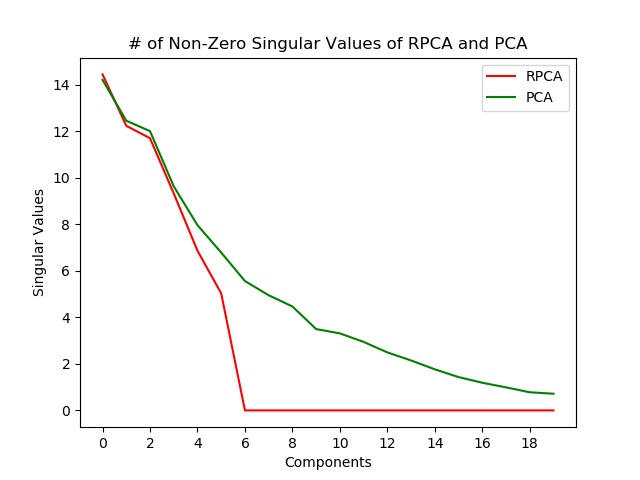
\includegraphics[width=50mm, scale=0.5]{Singular_Value_Plot_Test_120AnomSize5.jpg}
    \caption{Singular Value comparison for PCA and RPCA on synthetic data with 3 percent anomalies of size 5}
    \label{fig:singvaltrain1205}
\end{figure}
\begin{figure}[H]
\begin{minipage}[b]{0.45\linewidth}
    \centering
    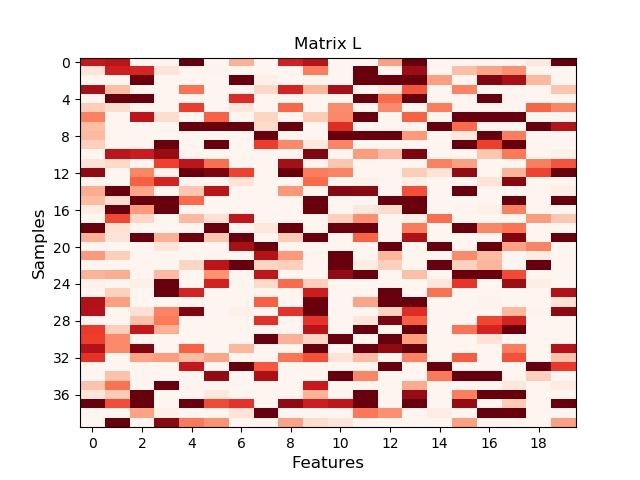
\includegraphics[width=45mm, scale=0.5]{L_120AnomSize5.jpg}
    \caption{Low-Rank Matrix resulting from RPCA on synthetic data with 3 percent anomalies of size 5}
    \label{fig:Ltrain1205}
\end{minipage}
\quad
\begin{minipage}[b]{0.45\linewidth}
    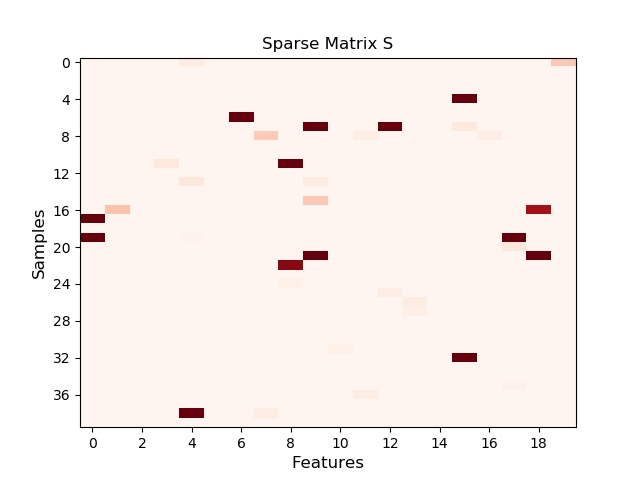
\includegraphics[width=45mm, scale=0.5]{S_120AnomSize5.jpg}
    \caption{Sparse Matrix resulting from RPCA on synthetic data with 3 percent anomalies of size 5}
    \label{fig:Strain1205}
\end{minipage}
\end{figure}

\begin{figure}[H]
\begin{minipage}[b]{0.45\linewidth}
    \centering

    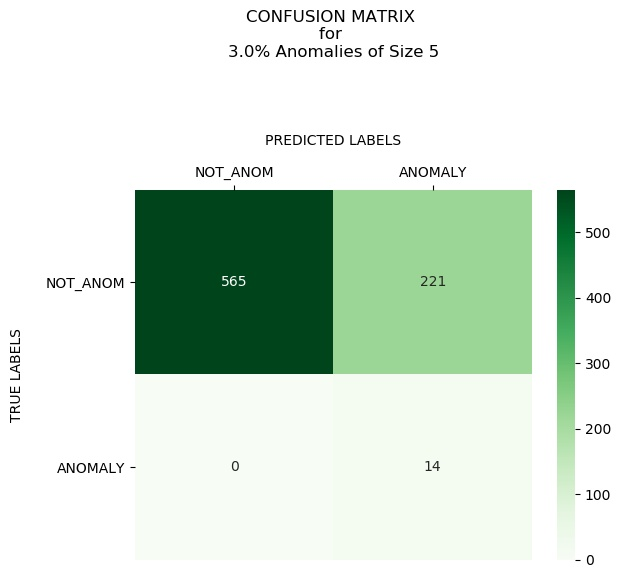
\includegraphics[width=50mm, scale=0.5]{cmPCATest_120AnomSize5.jpg}
    \caption{Confusion Matrix resulting from PCA on synthetic data with 3 percent anomalies of size 5}
    \label{fig::CMtrainPCA1205}
\end{minipage}
\quad
\begin{minipage}[b]{0.45\linewidth}
    \centering
    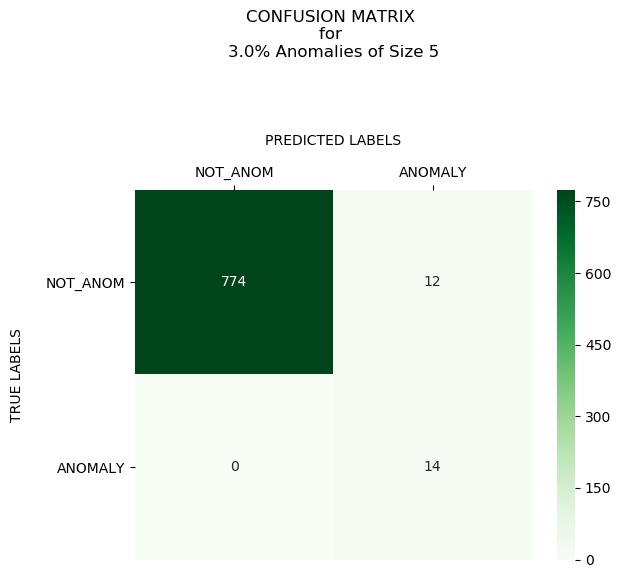
\includegraphics[width=50mm, scale=0.5]{cmRPCATest_120AnomSize5.jpg}
    \caption{Confusion Matrix resulting from RPCA on synthetic data with 3 percent anomalies of size 5}
    \label{fig::CMtrainRPCA125}
\end{minipage}
\end{figure}

% Insert Figures for three percent anomalies size 10

\begin{figure}[H]
    \centering
    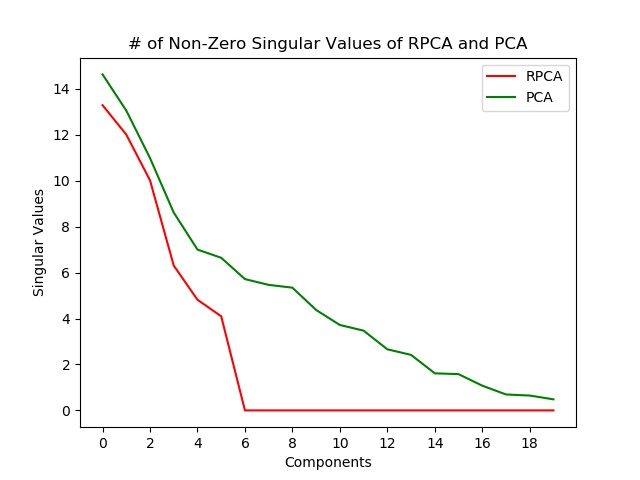
\includegraphics[width=50mm, scale=0.5]{Singular_Value_Plot_Test_120AnomSize10.jpg}
    \caption{Singular Value comparison for PCA and RPCA on synthetic data with 3 percent anomalies of size 10}
    \label{fig:singvaltrain12010}
\end{figure}
\begin{figure}[H]
\begin{minipage}[b]{0.45\linewidth}
    \centering
    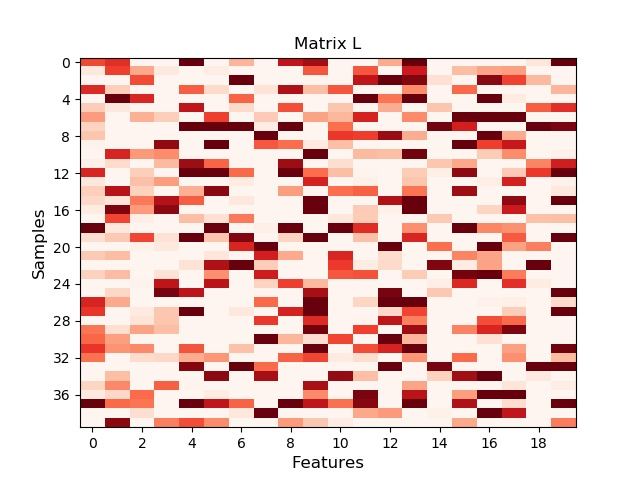
\includegraphics[width=45mm, scale=0.5]{L_120AnomSize10.jpg}
    \caption{Low-Rank Matrix resulting from RPCA on synthetic data with 3 percent anomalies of size 10}
    \label{fig:Ltrain12010}
\end{minipage}
\quad
\begin{minipage}[b]{0.45\linewidth}
    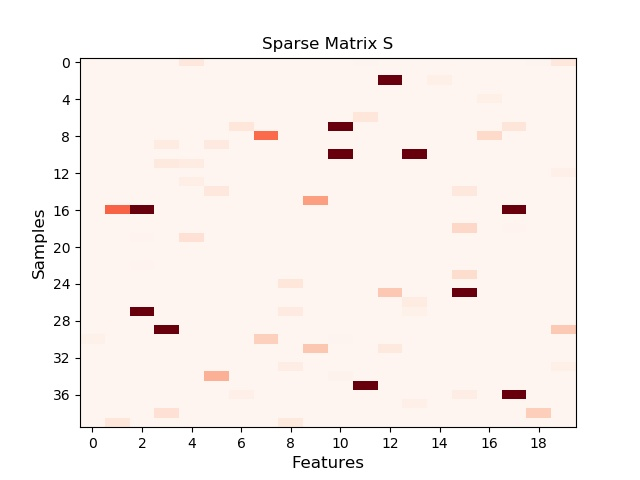
\includegraphics[width=45mm, scale=0.5]{S_120AnomSize10.jpg}
    \caption{Sparse Matrix resulting from RPCA on synthetic data with 3 percent anomalies of size 10}
    \label{fig:Strain12010}
\end{minipage}
\end{figure}

\begin{figure}[H]
\begin{minipage}[b]{0.45\linewidth}
    \centering

    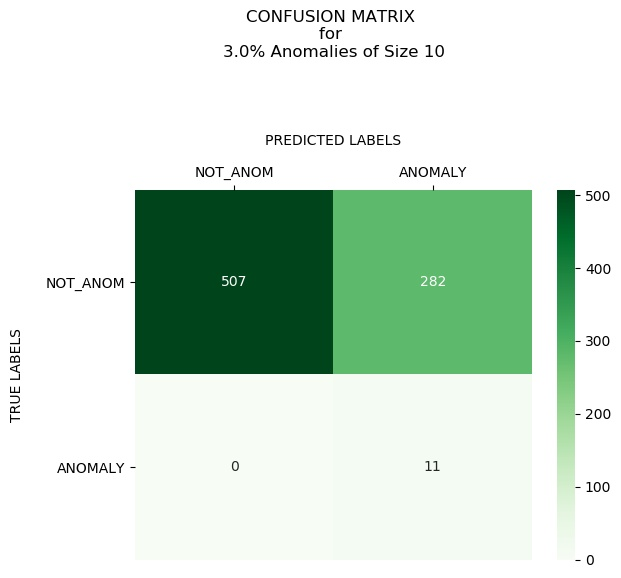
\includegraphics[width=50mm, scale=0.5]{cmPCATest_120AnomSize10.jpg}
    \caption{Confusion Matrix resulting from PCA on synthetic data with 3 percent anomalies of size 10}
    \label{fig::CMtrainPCA12010}
\end{minipage}
\quad
\begin{minipage}[b]{0.45\linewidth}
    \centering
    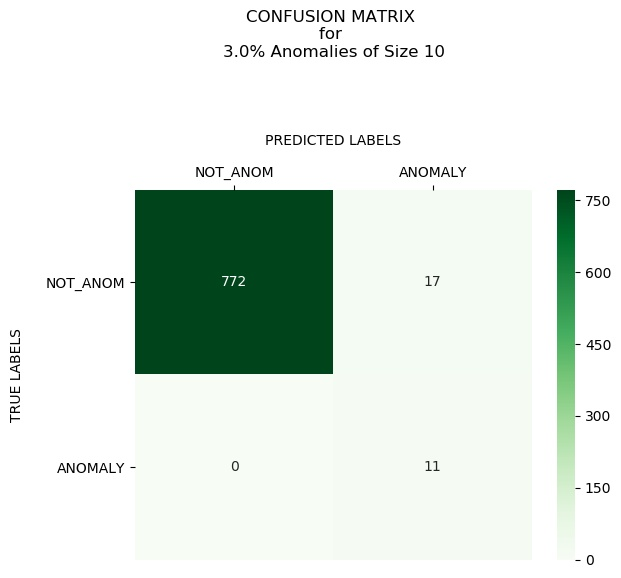
\includegraphics[width=50mm, scale=0.5]{cmRPCATest_120AnomSize10.jpg}
    \caption{Confusion Matrix resulting from RPCA on synthetic data with 3 percent anomalies of size 10}
    \label{fig::CMtrainRPCA12010}
\end{minipage}
\end{figure}

% Insert Figures for ten percent anomalies size 5

\begin{figure}[H]
    \centering
    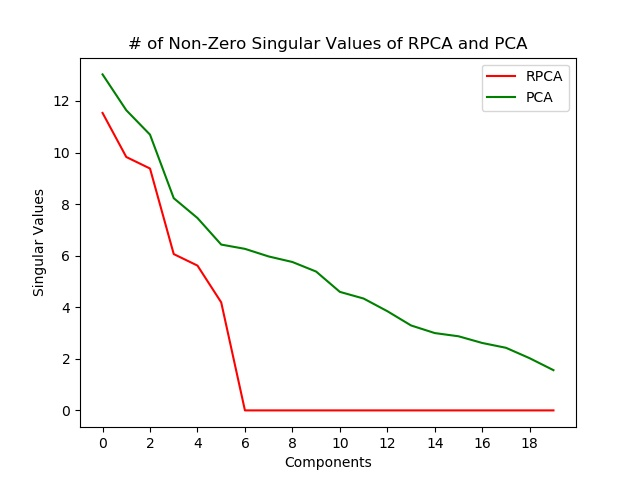
\includegraphics[width=50mm, scale=0.5]{Singular_Value_Plot_Test_400AnomSize5.jpg}
    \caption{Singular Value comparison for PCA and RPCA on synthetic data with 10 percent anomalies of size 5}
    \label{fig:singvaltrain4005}
\end{figure}
\begin{figure}[H]
\begin{minipage}[b]{0.45\linewidth}
    \centering
    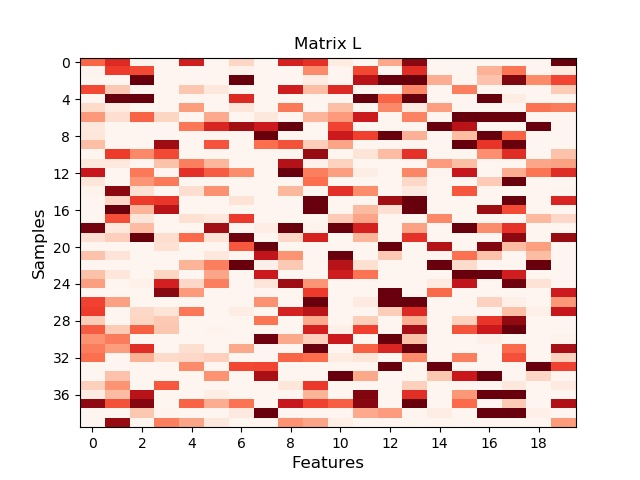
\includegraphics[width=45mm, scale=0.5]{L_400AnomSize5.jpg}
    \caption{Low-Rank Matrix resulting from RPCA on synthetic data with 10 percent anomalies of size 5}
    \label{fig:Ltrain4005}
\end{minipage}
\quad
\begin{minipage}[b]{0.45\linewidth}
    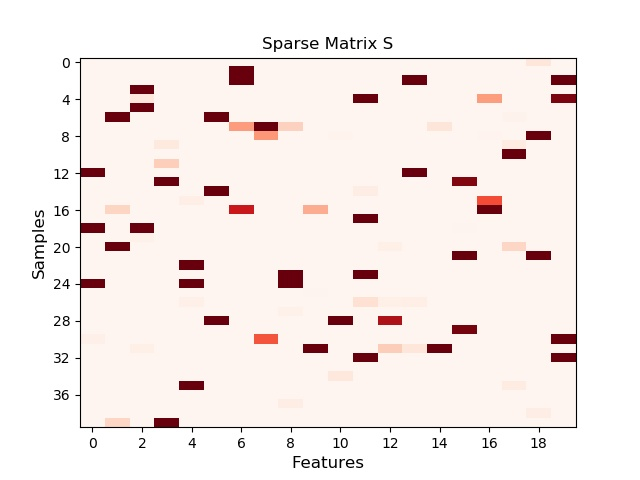
\includegraphics[width=45mm, scale=0.5]{S_400AnomSize5.jpg}
    \caption{Sparse Matrix resulting from RPCA on synthetic data with 10 percent anomalies of size 5}
    \label{fig:Strain4005}
\end{minipage}
\end{figure}

\begin{figure}[H]
\begin{minipage}[b]{0.45\linewidth}
    \centering

    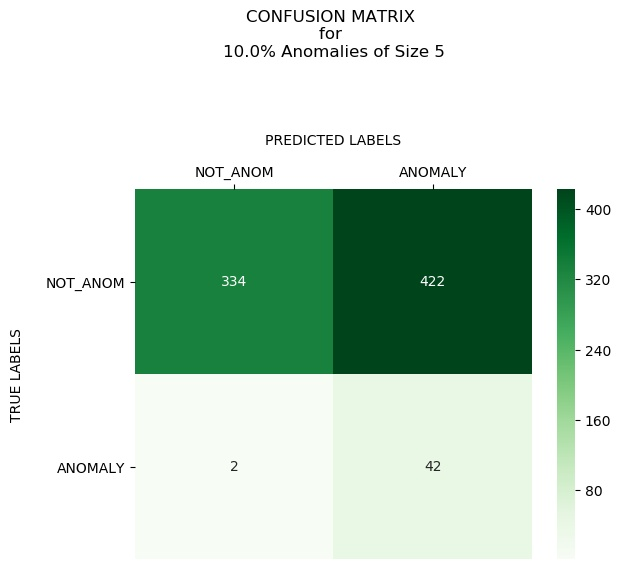
\includegraphics[width=50mm, scale=0.5]{cmPCATest_400AnomSize5.jpg}
    \caption{Confusion Matrix resulting from PCA on synthetic data with 10 percent anomalies of size 5}
    \label{fig::CMtrainPCA4005}
\end{minipage}
\quad
\begin{minipage}[b]{0.45\linewidth}
    \centering
    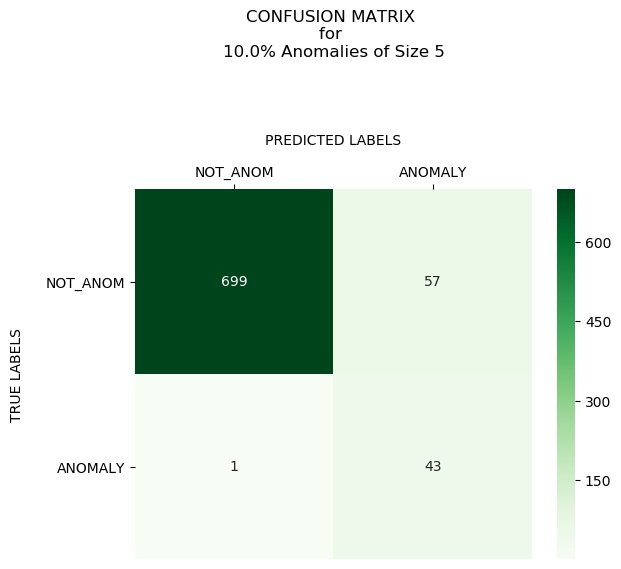
\includegraphics[width=50mm, scale=0.5]{cmRPCATest_400AnomSize5.jpg}
    \caption{Confusion Matrix resulting from RPCA on synthetic data with 10 percent anomalies of size 5}
    \label{fig::CMtrainRPCA4005}
\end{minipage}
\end{figure}

% Insert Figures for ten percent anomalies size 10

\begin{figure}[H]
    \centering
    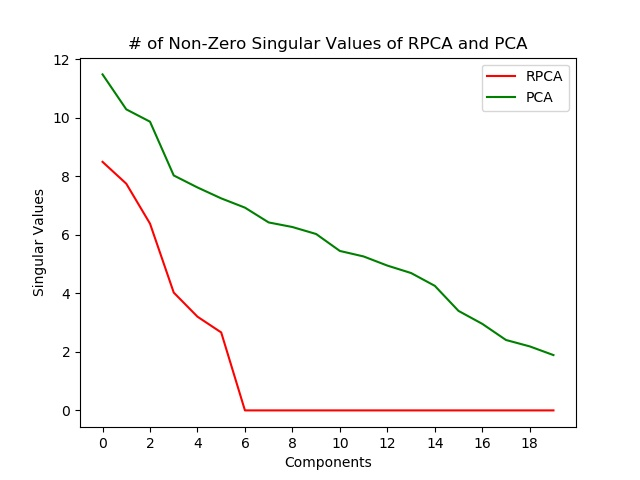
\includegraphics[width=50mm, scale=0.5]{Singular_Value_Plot_Test_400AnomSize10.jpg}
    \caption{Singular Value comparison for PCA and RPCA on synthetic data with 10 percent anomalies of size 10}
    \label{fig:singvaltrain40010}
\end{figure}
\begin{figure}[H]
\begin{minipage}[b]{0.45\linewidth}
    \centering
    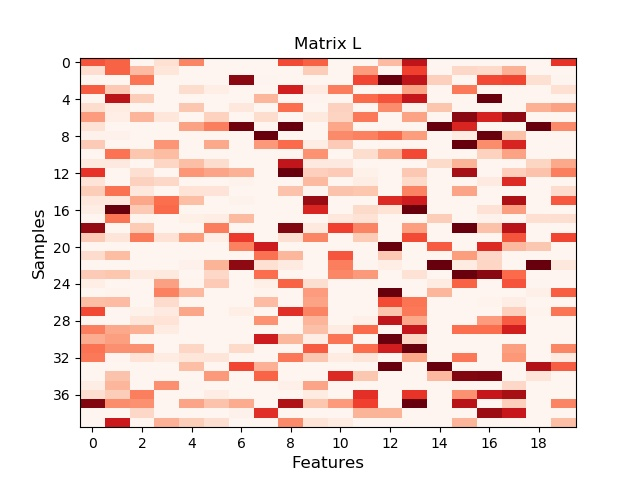
\includegraphics[width=45mm, scale=0.5]{L_400AnomSize10.jpg}
    \caption{Low-Rank Matrix resulting from RPCA on synthetic data with 10 percent anomalies of size 10}
    \label{fig:Ltrain40010}
\end{minipage}
\quad
\begin{minipage}[b]{0.45\linewidth}
    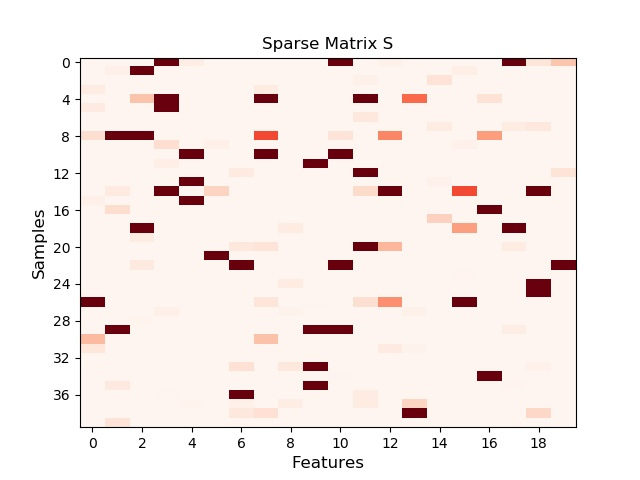
\includegraphics[width=45mm, scale=0.5]{S_400AnomSize10.jpg}
    \caption{Sparse Matrix resulting from RPCA on synthetic data with 10 percent anomalies of size 10}
    \label{fig:Strain40010}
\end{minipage}
\end{figure}

\begin{figure}[H]
\begin{minipage}[b]{0.45\linewidth}
    \centering

    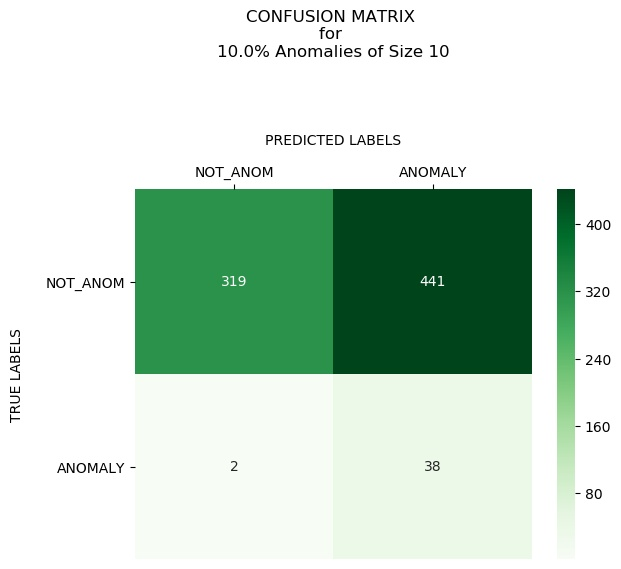
\includegraphics[width=50mm, scale=0.5]{cmPCATest_400AnomSize10.jpg}
    \caption{Confusion Matrix resulting from PCA on synthetic data with 10 percent anomalies of size 10}
    \label{fig::CMtrainPCA40010}
\end{minipage}
\quad
\begin{minipage}[b]{0.45\linewidth}
    \centering
    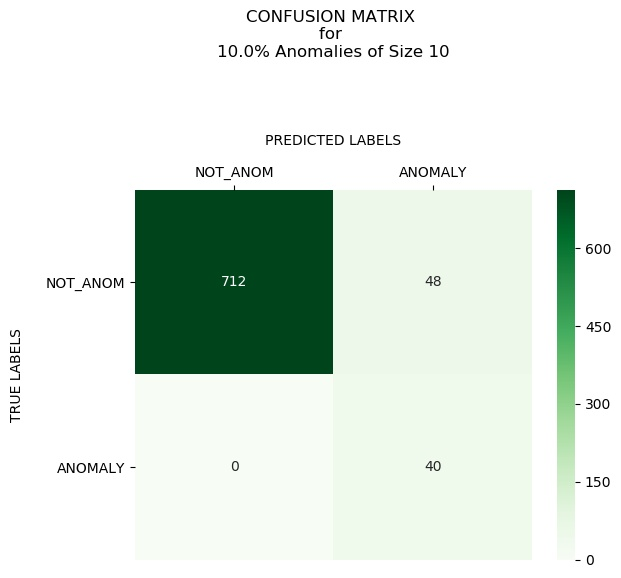
\includegraphics[width=50mm, scale=0.5]{cmRPCATest_400AnomSize10.jpg}
    \caption{Confusion Matrix resulting from RPCA on synthetic data with 10 percent anomalies of size 10}
    \label{fig::CMtrainRPCA40010}
\end{minipage}
\end{figure}

\todo[inline]{Add MSE plots of outliers against error plot data csv files}
\todo[inline]{Add results for Deon's combinatorial approach}

\subsection{Real Data}
\subsubsection{Data Description}

The health data set that we chose to analyze was provided by the Centers for Medicare and Medicaid Services (CMS). The public use file is available at CMS.gov and contains data related to the Shared Savings Program Accountable Care Organizations (ACO) in the year 2016. The dataset consists of 432 ACOs and makes use of 34 nationally recognized Quality Measures.  A simple boxplot visualization of the normalized dataset reveals the distributions, skewed data and outliers of the various features. It is not unusual for real world data to be noisy and impacted by outliers due to human error, but it does complicate analysis.\\

\begin{figure}[H]
    \centering
    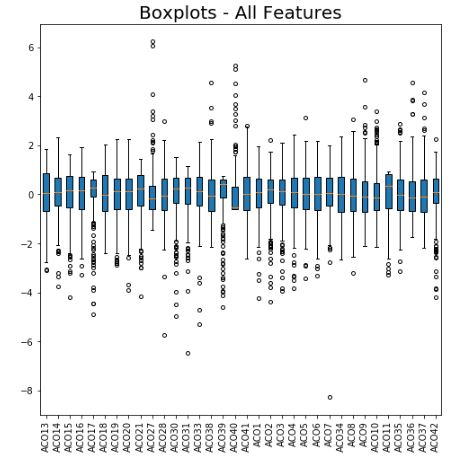
\includegraphics{BoxPlots_ALL.jpg}
    \caption{Boxplot of all features}
    \label{fig:boxall}
\end{figure}

The quality measures can be divided into distinct sub-categories. Boxplots created for each of these categories may reveal differences in the data distributions for each category of features. The GPRO features in particular appear to have greater variability and larger outliers.

\begin{enumerate}
\item GPRO - Group Practice Reporting Option Features (16 measures) : GPRO features are collected by a web interface which was designed specifically to capture ACO-reported clinical quality data.

\begin{figure}[H]
    \centering
    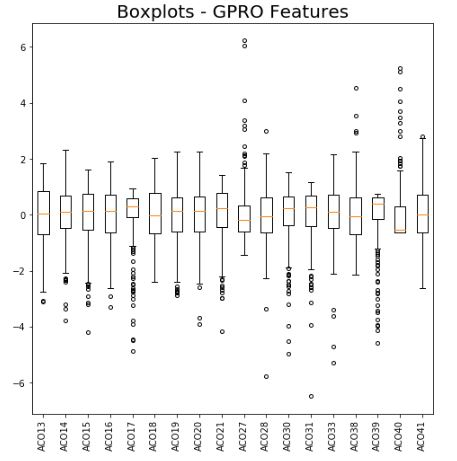
\includegraphics{BoxPlots_GPRO.jpg}
    \caption{Boxplot of GPRO features}
    \label{fig:boxgpro}
\end{figure}


\item CAHPS - Consumer Assessment of Healthcare Providers Features (10 measures) : CAHPS features are collected by a survey administered by a CMS-approved vendor selected and paid for by individual ACOs.

\begin{figure}[H]
    \centering
    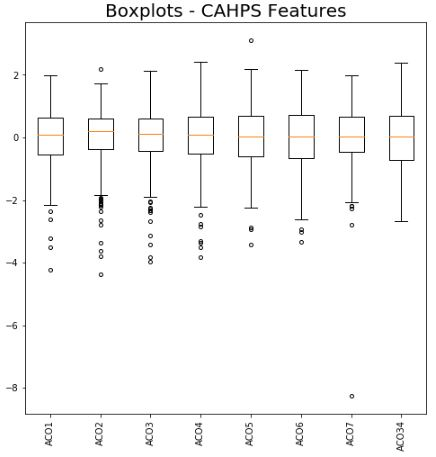
\includegraphics{BoxPlots_CAHPS.jpg}
    \caption{Boxplot of CAHPS features}
    \label{fig:boxcahps}
\end{figure}

\item EHR - Electronic Health Record Features (8 measures) : EHR features are calculated by the CMS ACO PAC based on CMS claims and administrative data extracted from the National Level Repository. 
\end{enumerate}

\begin{figure}[H]
    \centering
    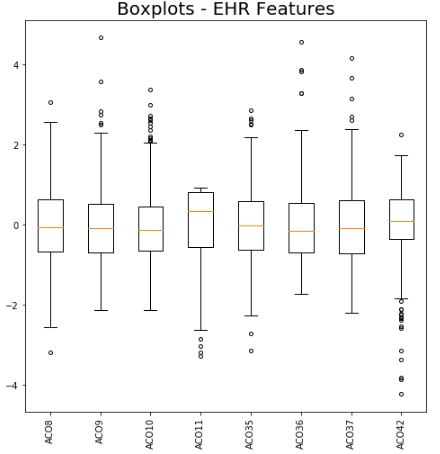
\includegraphics{BoxPlots_EHR.jpg}
    \caption{Boxplot of EHR features}
    \label{fig:boxehr}
\end{figure}


\subsubsection{Approach}
\todo[inline]{Add approach for real data}
\todo[inline]{Do Paffenroth insertions: add anomalies and show that we found them}
\subsubsection{Results}
\todo[inline]{Add results for real data: What does PCA/RPCA/Gurobi find}

\section{Conclusions}

"This work suggests a new research path to explore how modern optimization methods can help complement medical and policy judgement when seeking to select health metrics from a proposed set of candidates when there is reason to expect menasurement errors and varying burden levels in the data collection process." Data analytics methods are particularly valuable for comparing various subsets of metrics when accounting for anomalies and noise due to human and measurement error. [Ref AcademyHealth Abstract]
\todo[inline]{Create a proper bibliography}
\newpage
\listoftodos[Notes]
\end{document}